

%    ____                    __  _____                       __  _           
%   / __/__  ___________ ___/ / / ___/__  ___ _  _____  ____/ /_(_)__  ___   
%  / _// _ \/ __/ __/ -_) _  / / /__/ _ \/ _ \ |/ / -_)/ __/ __/ / _ \/ _ \_ 
% /_/  \___/_/  \__/\__/\_,_/  \___/\___/_//_/___/\__/\__/\__/_/\___/_//_(_)




\section{Estudio de Convección por Semejanza}
\subsection{Correlación empírica para Convección Natural}
\begin{figure}[htb!]
    \centering
    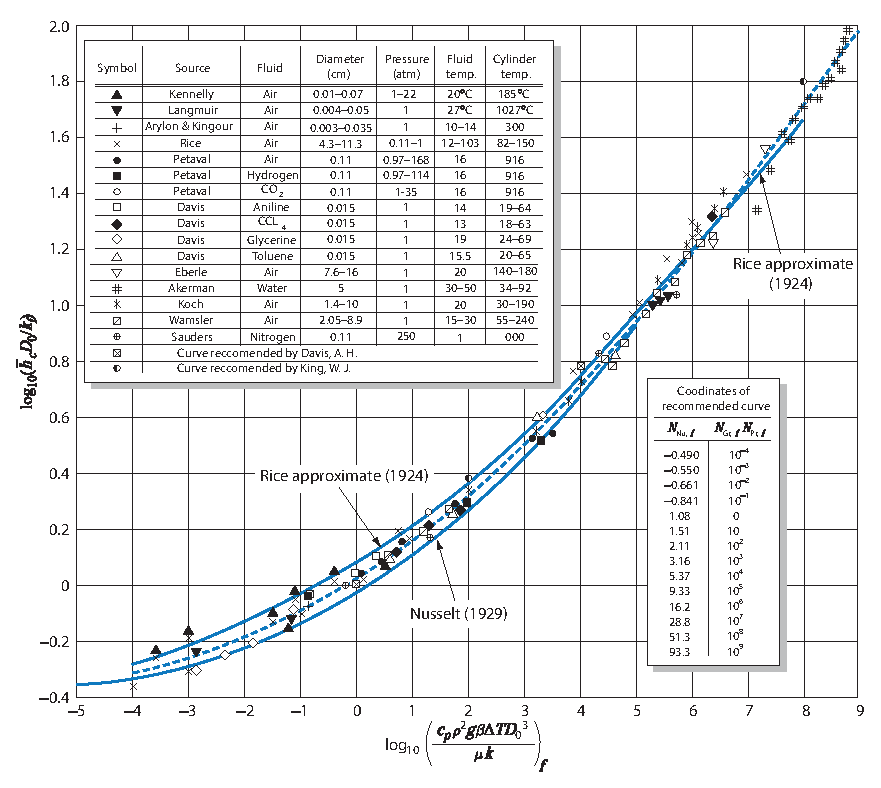
\includegraphics[width=\textwidth/2]{graf.eps}
    \caption{Correlación empírica para transferencia de calor en cilindros horizontales con gases y líquidos.\cite{kreith2011principles}}
    \label{graf:NusseltNaturalConvectionHorizontalCilinder}
\end{figure}
\begin{figure}[htb!]
    \centering
    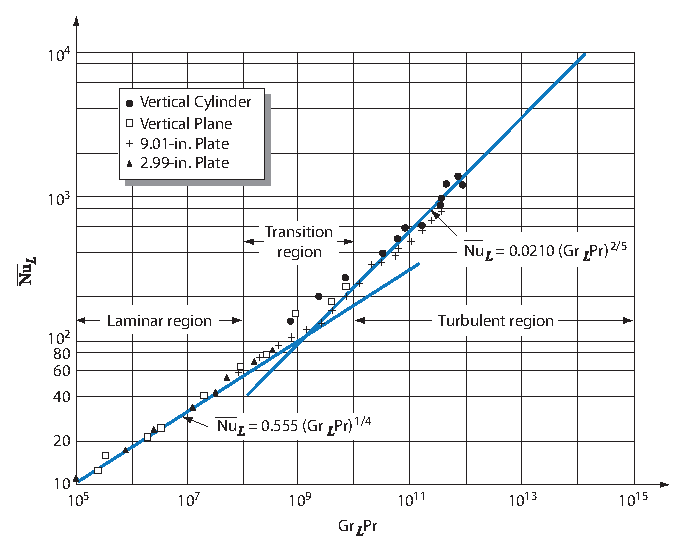
\includegraphics[width=\textwidth/2]{plaque.eps}
    \caption{Correlación empírica para transferencia de calor en cilindros y placas \emph{verticales}. \cite{kreith2011principles}}
    \label{graf:NusseltNaturalConvectionVerticalCilinderPlate}
\end{figure}
\subsubsection{Placas verticales}
Esta sección va exponer relaciones que coinciden con la realidad. Como en el Kreith, la dimensión característica aparece como subíndice para los parámetros adimensionales ($\Nusselt$, $\Reynolds$ etc.)

Placa o cilindro isotérmico vertical a una distancia $x$ de su comienzo con su capa limite
\begin{align*}\numberthis \label{eq:VerticalPlateOrCilinderPoint}
    h_{cx}&=0,508\Prandtl^{\frac{1}{2}}\sqrt[4]{\frac{\Grashof_x}{0,952+\Prandtl}}\frac{k}{x}\\
    \delta(x)&=4,3x\sqrt[4]{\frac{\Prandtl+0,56}{\Prandtl^2 \Grashof_x}}
\end{align*}
Integrando sobre la longitud característica $L$ y dividiendo por $L$ se puede obtener $\hcb=0,68\Prandtl^{\frac{1}{2}}\sqrt[4]{\frac{\Grashof_L}{0,952+\Prandtl}}\frac{k}{L}$.

Para una superficie plana sumergida en un metal fundido ($\Prandtl<0,03$) el promedio del número de $\Nusselt$ es
\begin{equation}
    \overline{\Nusselt}_L= \frac{\hcb L}{k}=0,68\sqrt[3]{\Grashof_L \Prandtl^2}
\end{equation}

en cambio, para régimen turbulento ($\Grashof>\num{e9}$) se recomienda:
\begin{equation}
    \overline{\Nusselt}_L=\frac{\hcb L}{k}=0,13\sqrt[3]{\Grashof \Prandtl}
\end{equation}

Para una placa inclinada a $\theta$ en el rango $\num{e5}<\Grashof_L\Prandtl\cos\theta<\num{e11}$ y $0\leq\theta\leq 89\grados $.
\begin{equation}
    \overline{\Nusselt_L}=0,56(\Grashof_L \Prandtl \cos\theta)
\end{equation}
\subsubsection{Placas horizontales}
Se tienen dos casos, cuando la gravedad ayuda a la transferencia de calor (\ref{eq:HorizontalPlateGravityHelping}) y cuando le juega en contra (\ref{eq:HorizontalPlateGravityBeingABitch}) donde $\ell$ toma el valor representativo $\frac{\textrm{Area de superficie}}{\textrm{Perímetro}}$:

\begin{align*}\numberthis\label{eq:HorizontalPlateGravityHelping}
    \overline{\Nusselt}_\ell &=0,54\sqrt[4]{\Rayleigh_\ell} \qquad (\num{e5}\lessapprox\Rayleigh_\ell \lessapprox\num{e7})\\
    \overline{\Nusselt}_\ell&=0,15\sqrt[3]{\Rayleigh_\ell} \qquad (\num{e7}\lessapprox\Rayleigh_\ell\lessapprox \num{e10})\\
\end{align*}
\begin{equation}\label{eq:HorizontalPlateGravityBeingABitch}
    \overline{\Nusselt}_\ell=0,27\sqrt[4]{\Rayleigh_\ell} \qquad (\num{e5}\lessapprox\Rayleigh_\ell \lessapprox \num{10e10})
\end{equation}




\subsection{Correlación empírica para cuerpos no-fuselados o \emph{bluff} con Convección forzada}
\textbf{Cuerpo no-fuselado}:\emph{Un cuerpo que tiene el frente ancho, aplanado, como en el caso de algunos vehículos de reentrada atmosférica.} 

\subsubsection{Cilindros}
$$C_D=\frac{F_D}{A_f\left( \rho U^2_\infty /2g_c\right)}$$
donde $D$ es el diámetro exterior, $L$ es la longitud del cilindro, $A_f$ es el área frontal proyectado,$U_\infty$ es la velocidad de la corriente libre.

Para un cilindro se puede calcular $h_c$ sobre un punto cualquiera a $\theta$ grados de la horizontal que \emph{enfrenta} el flujo \textbf{laminar adherido}. 
\begin{equation} \label{eq:nusselt}
    \Nusselt_D(\theta)=\frac{h_c(\theta) D}{k}=1,14\sqrt{\frac{\rho U_\infty D}{\mu}}\cdot \Prandtl^{0.4} \left[ 1- \left(\frac{\theta}{90}\right)^3 \right] 
\end{equation}
El coeficiente de transferencia de calor es máximo en el punto estancamiento que enfrenta al flujo. A números de Reynolds mas altos se generan eddies en la parte posterior del cilindro que no mezclan efectivamente con el flujo principal disminuyendo así la transferencia de calor en $\theta=180$.

El problema se vuelve complejo para Reynolds altos. 
\begin{equation} \label{eq:nusseltmean}
    \overline{\Nusselt}_D=\frac{\hcb D}{k}=C\left(\frac{U_\infty D}{\nu}\right)^m \Prandtl^n \left( \frac{\Prandtl}{\Prandtl_s}\right)^{0.25}
\end{equation}
evaluado con $n=0,37$ para $\Prandtl<10$ y $n=0,36$ para $\Prandtl>10$ 

\begin{table}[h]
\centering
\begin{tabular}{ccc}
\hline
$\Reynolds$                & C     & m   \\\hline
$1$ -- $40$              & $0,75$  & $0,4$ \\
$40$ -- $\num{1e3}$           & $0,51$  & $0,5 $\\
$\num{1e3}$ -- $\num{2e5}$      & $0,26$  & $0,6$ \\
$\num{2e5}$ -- $\num{1e6}$ & $0,076$ & $0,7$\\\hline
\end{tabular}
\label{tab:coeficientes1}
\caption{Coeficientes para la ecuación \ref{eq:nusseltmean}}
\end{table}

Si se tiene un cilindro que no esta en \emph{cross-flow} (caso $\vartheta=90\grados$ siendo $\vartheta$ el ángulo de \emph{guiñada} o \emph{yaw angle}):
\begin{equation}
    \overline{\Nusselt}_D=0,206\Reynolds^{0,63}_N \Prandtl^{0.36} \qquad 2500<\Reynolds_N<\Reynolds_\crit
\end{equation}
donde $\Reynolds_N=\Reynolds_D \sin \vartheta $ y $\Reynolds_\crit$ varía dependiendo de $\vartheta$ entre \num{2e4} para $\vartheta=15\grados$ y \num{2.5e5} para $\vartheta=45\grados$

En el rango $\num{2e5}<\Reynolds_D<\num{e6}$ el número de Nusselt es independiente de $\vartheta$
\begin{equation}
    \overline{\Nusselt}_D=0,012\Reynolds_D^{0,85}\Prandtl^{0,36}
\end{equation}

Un cuerpo prismático de sección no-circular en un medio gaseoso se puede describir con siguiente ecuación tomando $B$ y $n$ de tabla
\begin{equation}
    \overline{\Nusselt}_D=B\Reynolds_D^n
\end{equation}

Usar $\Nusselt_D=1,125\left( \Reynolds_D \Prandtl\right)^{0,413}$ para cilindros con flujo metal-liquido $\vartheta=90\grados$. Valido en el rango $1\leq\Prandtl\cdot \Reynolds_D\leq 100$. 

El \emph{aspect ratio} $\frac{L}{D}$ juega un rol para valores menores a $4$. Dentro de este rango y para valores de Reynolds $\num{7e4} < \Reynolds_D < \num{2.2e5}$
\begin{equation}
    \overline{\Nusselt}_D=0,123 \Reynolds_D^{0,651}+0,00416\left( \frac{L}{D} \right)^{-0,85} \Reynolds_D^{0,792}
\end{equation}b

\subsubsection{Esferas}
En el rango $25 < \Reynolds_D < \num{1e5}$ vale la siguiente ecuación para una esfera calentada o enfriada por un gas:
\begin{equation} \label{eq:nusseltspheregas}
    \overline{\Nusselt}_D=\frac{\bar{h}_cD}{k}=0,37\left( \frac{\rho D U_\infty}{\mu}\right)^{0,6}=0,37\Reynolds_D^{0,6} 
\end{equation}

Para un flujo de un \textbf{gas} $1,0<\Reynolds_D<25$:
\begin{equation}
    \hcb = c_pU_\infty \rho \left(\frac{2,2}{\Reynolds_D}+\frac{0,48}{\sqrt{\Reynolds_D}} \right)
\end{equation}

Si se quisiera modelar la transferencia de calor en un liquido (o un gas) para $3.5<\Reynolds_D<\num{7.6e4}$ y $0,7<\Prandtl<380$:

\begin{equation}
    \overline{\Nusselt}_D\!=\frac{\hcb D}{k}=2+\!\left(0,4 \sqrt{\Reynolds_D}+\!0,06\sqrt[3]{\Reynolds_D^2}\right) \Prandtl^{0,4}\sqrt[4]{\frac{\mu}{\mu_s}}
\end{equation}
donde $\mu_s$ es la viscosidad del fluido a la temperatura de la superficie de la esfera.

Por debajo del $\Reynolds_\crit$,  $100<\Reynolds_D<\num{2e5}$ la ecuación anterior es modificada:
\begin{equation}\label{eq:nusseltspheresubcrit}
    \overline{\Nusselt}_D=2+\left( \frac{\Reynolds_D}{4}+\num{3e-4}\Reynolds_D^{1,6}\right)^\frac{1}{2}
\end{equation}

Después del limite critico (seguimos con gases) $\num{4e5}<\Reynolds_D<\num{5e6}$ con $a=\num{5e-3}$, $b=\num{2,5e-10}$ y $c=\num{-3,1e-17}$
\begin{equation}
    \overline{\Nusselt}_D=430+a\Reynolds_D+b\Reynolds_D^2+c\Reynolds_D^3
\end{equation}

Ahora en el caso que se esté transfiriendo calor de una esfera a un metal liquido en el rango $\num{3.6e4}<\Reynolds_D<\num{2e5}$ tenemos:
\begin{equation}
    \overline{\Nusselt}_D=\frac{\hcb D}{k}=2+0,386 \left( \Reynolds_D \Prandtl\right)^{\frac{1}{2}}
\end{equation}

\subsubsection{Otros objetos no-fuselados}
Números de Nusselt para una placa plana de ancho $D$ normal al flujo incidente (\ref{eq:nusseltplacaplana}) y un cilindro de sección semi-circular (lado curvo enfrentando el flujo) (\ref{eq:nusseltsemicilindro}) para $1,0<\Reynolds_D<\num{4e5}$:
\begin{equation}\label{eq:nusseltplacaplana}
    \overline{\Nusselt}_D=\frac{\hcb D}{k}=0,20\Reynolds^{\frac{2}{3}}_D
\end{equation}
\begin{equation}\label{eq:nusseltsemicilindro}
    \overline{\Nusselt}_D=\frac{\hcb D}{k}=0,16\Reynolds^{\frac{2}{3}}_D
\end{equation}

Para un disco orientado con su eje en la dirección de un flujo, valido en $5000<\Reynolds_D<\num{5e4}$:
\begin{equation}
    \overline{\Nusselt}_D=1,05\Reynolds_D^{\frac{1}{2}} \Prandtl^{0,36}
\end{equation}

Los datos experimentales obtenidos para una placa cuadrada orientada con guiñada $\vartheta\in [0\grados,45\grados]$ y ángulo de ataque $\vartheta_{\textrm{pitch}}\in[25\grados,90\grados]$ increíblemente tiene correlación con una sola ecuación (error=$\pm 5\%$):
\begin{equation}
    \frac{\hcb \Prandtl^{\frac{2}{3}}}{c_p\rho U_\infty}=\frac{0,930}{\sqrt{\Reynolds_L}}
\end{equation}
